\usepackage{tikz-dependency}

\title[Digital Methods]{Applied Quantitative Text Analysis\\@ Digital Methods Workshop}

\author[Joel Nothman]{Joel Nothman\\\texttt{\small joel.nothman@sydney.edu.au}}
\institute{Sydney Informatics Hub\\University of Sydney}
\date{8th June, 2018}

\setbeamersize{text margin left=20pt, text margin right=20pt, description width=50pt}

\usepackage{LI}
%\usepackage{syntree}

\newcommand{\ex}[1]{\textcolor{usydblue}{#1}}
\newcommand{\glow}[1]{\textcolor{usydred}{#1}}

\usepackage{stackengine}
\usepackage{scalerel}
\usepackage{xcolor}
\newcommand\dangersign[1][2ex]{%
  \renewcommand\stacktype{L}%
  \scaleto{\stackon[1.3pt]{\color{red}$\triangle$}{\tiny\bfseries !}}{#1}%
}

\begin{document}

\titleslide

\iffalse
\begin{points}{Who am I?}
	\p PhD in natural language processing @ USyd\\
	   on modelling reference to events in news
	\p Data science research engineer with the Sydney Informatics Hub
	\p Lecture Natural Language Processing (COMP5046)\\
	   for the School of Information Technologies
	\p Volunteer software engineer for popular data science and language processing tools
\end{points}
\fi

\section{Language}

\begin{points}{Language can tell us a lot about people}
	\p how do people \glow{feel} about some product / event / situation?
	\p why do people \glow{share} some media?
	\p how do people \glow{persuade} or negotiate?
	\p how do people express their \glow{identity} as a community member?
	\p how do people, communities and periods \glow{differ} from one another?
	\vfill
	\p studying these questions: content analysis, discourse analysis, corpus linguistics \ldots
	\vfill
	\p treating language as data might not be straightforward
	\vfill
\end{points}

\iffalse
\begin{points}{Characterising Trump's Android and iPhone tweets (0)}
	\p \href{http://varianceexplained.org/r/trump-tweets/}{Blog post by David Robinson (2016)}
	\p Hypothesis:
	\begin{itemize}
			\p only some of Trump's tweets are written by Trump
			\p these are distinguishable by the app doing the tweeting
			\p there are marked differences in communication style and message
			\p these may reflect different political intentions
	\end{itemize}
	\p Goal: characterise regular differences between Android and iPhone-posted tweets from @realDonaldTrump
\end{points}
\fi

\begin{points}{Language is \ldots}
	\p \glow{structured}: \ex{Jack kicked Jill} $\ne$ \ex{Jill kicked Jack}% \\
%%%	(morphosyntactic structure; discourse structure)
	\p free to represent arbitrary \glow{meaning}% \\
%	(lexicon + composition $\approx$ semantics)
	\p an \glow{efficient} encoding of a communicative purpose \\
	given context, shared knowledge, and social convention % \\
%%%	(pragmatics)
	\p efficiently decoded by humans despite rife \glow{ambiguity}
	\p highly \glow{variable} over time, place and genre/purpose
\end{points}

\begin{points}{Ambiguity everywhere}
			% Great examples at http://cs.nyu.edu/faculty/davise/ai/ambiguity.html
			\p of lexical semantics: \ex{I walked to the bank}
			\p of structure: \ex{I saw the girl on the hill with the telescope}
%%%			\p with elision: \ex{John kissed his wife and so did Sam}
			\p of named entity reference: \ex{Washington} (George, Denzel, city, state, US government, university, sports teams, \ldots)
			\p of semantic roles: \ex{Jill's care} -- is Jill giver or recipient?
%%%			\p of anaphora: \ex{Jane called Susan's but \emph{she} didn't (get an) answer}
%%%			\hspace{2em}\ex{I had surgery yesterday. They told me to stay in bed.}
			\p \ldots
\end{points}


\begin{points}{Language is statistically sparse}
   \p infinitely many words/phrases/sentences; almost all are \glow{rare}
   \p many ways to express the same thing
			\p we ideally want equivalent analyses of
			\begin{itemize}
					 \p \ex{Google bought YouTube for \$1bn}
					 \p \ex{The tech giant's acquisition of YouTube for \$1bn}
					 \p \ex{YouTube, which was acquired by Google for \$1bn}
					 \p \ex{Google didn't hesitate to snatch it up for a billion bucks}
			\end{itemize}
		\p non-literal language: \ex{Canberra announced}; \ex{kicked the bucket}
	\vfill
	\p How do ambiguity and variety of expression affect working with langugage as data?
\end{points}

\iffalse
Some thoughts:




* retrieval
    - want to avoid costly manual labour in finding texts with relevant phenomena
    - (data scientists often frame this as a prediction problem too)

* prediction


    we have existing tools for prediction


You don't make a NLP problem: if you have or can get structured data that tells you roughly the same thing, don't try to do it through analysing language.



Text classification
Entity extraction
Relation extraction


Examples!!

\fi


\section{Goals}

\begin{points}{Objectives of text processing in research}
	\vfill
	\p \glow{description}\\ identify patterns in text
	\vfill
	\p \glow{retrieval}\\ find relevant content in a collection
	\vfill
	\p \glow{prediction}\\ automate labelling of textual phenomena
	\vfill
\end{points}

\begin{points}{Description}
	\p may involve \glow{comparing frequencies} of some textual features
	\begin{itemize}
		\p Does one president use \emph{I}, \emph{me} much more than another?
	   \p What distinguishes men's and women's tweets?
	\end{itemize}
	\p may involve \glow{finding clusters} of similar content
	\begin{itemize}
		\p What political parties, internationally, have similar platforms?
	\end{itemize}
	\p may involve \glow{visualising} patterns in a text collection
\end{points}

\begin{points}{Textual features}
	\p usually our research question is about \emph{content}/\emph{meaning} or \emph{style}
	\p but we need quantifiable properties of the text
	\vfill

    \p naive approaches to language  tend to be most interpretable
	\begin{itemize}
		\item comparing word (or n-gram) frequency
		\item sentiment polarity, LIWC
		\item syllables per word, words per sentence
	\end{itemize}
    \p but always validate your quantitative conclusions
	\begin{itemize}
		\item manual inspection: does the result mean what you think it means?
		\item statistical validation: will the result hold on new data?
	\end{itemize}
\end{points}

\begin{centre}{Findings should be validated by manual review} 
	A \glow{concordance} lists when a term appears, with surrounding context\\
	\href{https://books.google.com/ngrams}{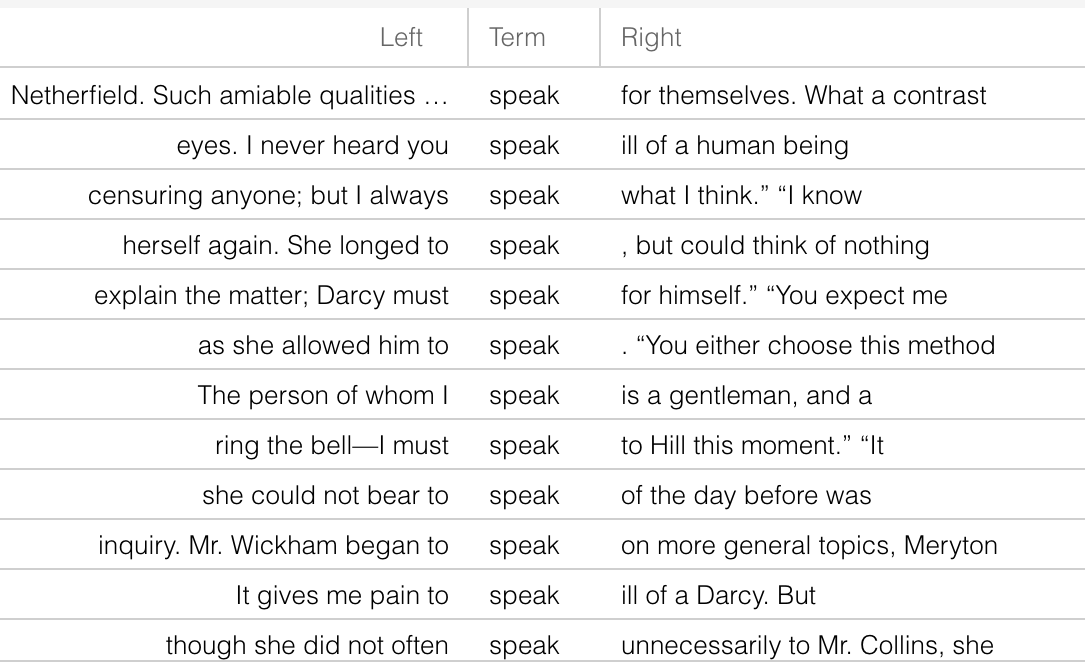
\includegraphics[width=.8\textwidth]{fig/concordance}}\\
	From \href{http://voyant-tools.org/}{Voyant Tools}
\end{centre}

\begin{points}{Retrieval}
    \p avoid manual labour of finding texts with relevant phenomena
	\begin{itemize}
		\p How did an idea spread through a social network?
	\end{itemize}
	\item may need be able to compute how similar two texts are
\end{points}

\begin{points}{Prediction}
	\item avoid manual labour of labelling some phenomenon
	\begin{itemize}
		   \p Can we work out if someone is happy from their words?
		   \p How typical is a speech of a particular political affiliation?
		   \p Replicate human judgements of writing quality
	\end{itemize}
	\item label a sample and try build an accurate system to label more
	\item model does not need to be interpretable, as long as it predicts well
	\item automated labelling may assist in description e.g.\ reducing the amount of manual coding in content analysis
\end{points}

\section{Prerequisites}

\begin{points}{Collecting text}
	\p We don't tend to start with tidy paragraphs
	\begin{itemize}
	\p Web forums with structure, quotation, signatures
	\p Online news with boilerplate
	\p Twitter
	\p PDFs with headers and footers
	\p Paper / microfiche
	\end{itemize}
	\vfill
	\p \glow{Cleaning} is inevitable
	\begin{itemize}
		\p Web scraping
		\p Boilerplate removal
		\p Optical character recognition
		\p Spam and duplicate removal
		\p Spelling correction or normalisation
	\end{itemize}
	\p Then need to \glow{tokenise} text into sentences and words
\end{points}

\begin{points}{Collections of cleaned text can be reused}
	\p A fixed collection of texts is a \glow{corpus} (plural \glow{corpora})
	\p To find unusually frequent words in someone's speech, you need to compare against an appropriate reference corpus
	\vfill
	\p General-purpose corpora select for:
	\begin{itemize}
		\p dialect (e.g.\ British National Corpus)
		\p genre (fiction, government, humour, news in Brown Corpus)
		\p medium (newswire, blogs, web forums, conversational speech, broadcast speech)
	\end{itemize}
	\vfill
%%%	\p Make your corpus representative of the phenomenon you are studying
\end{points}

\begin{centre}{Large scale corpora allow us to expore language variation}
	\href{https://books.google.com/ngrams}{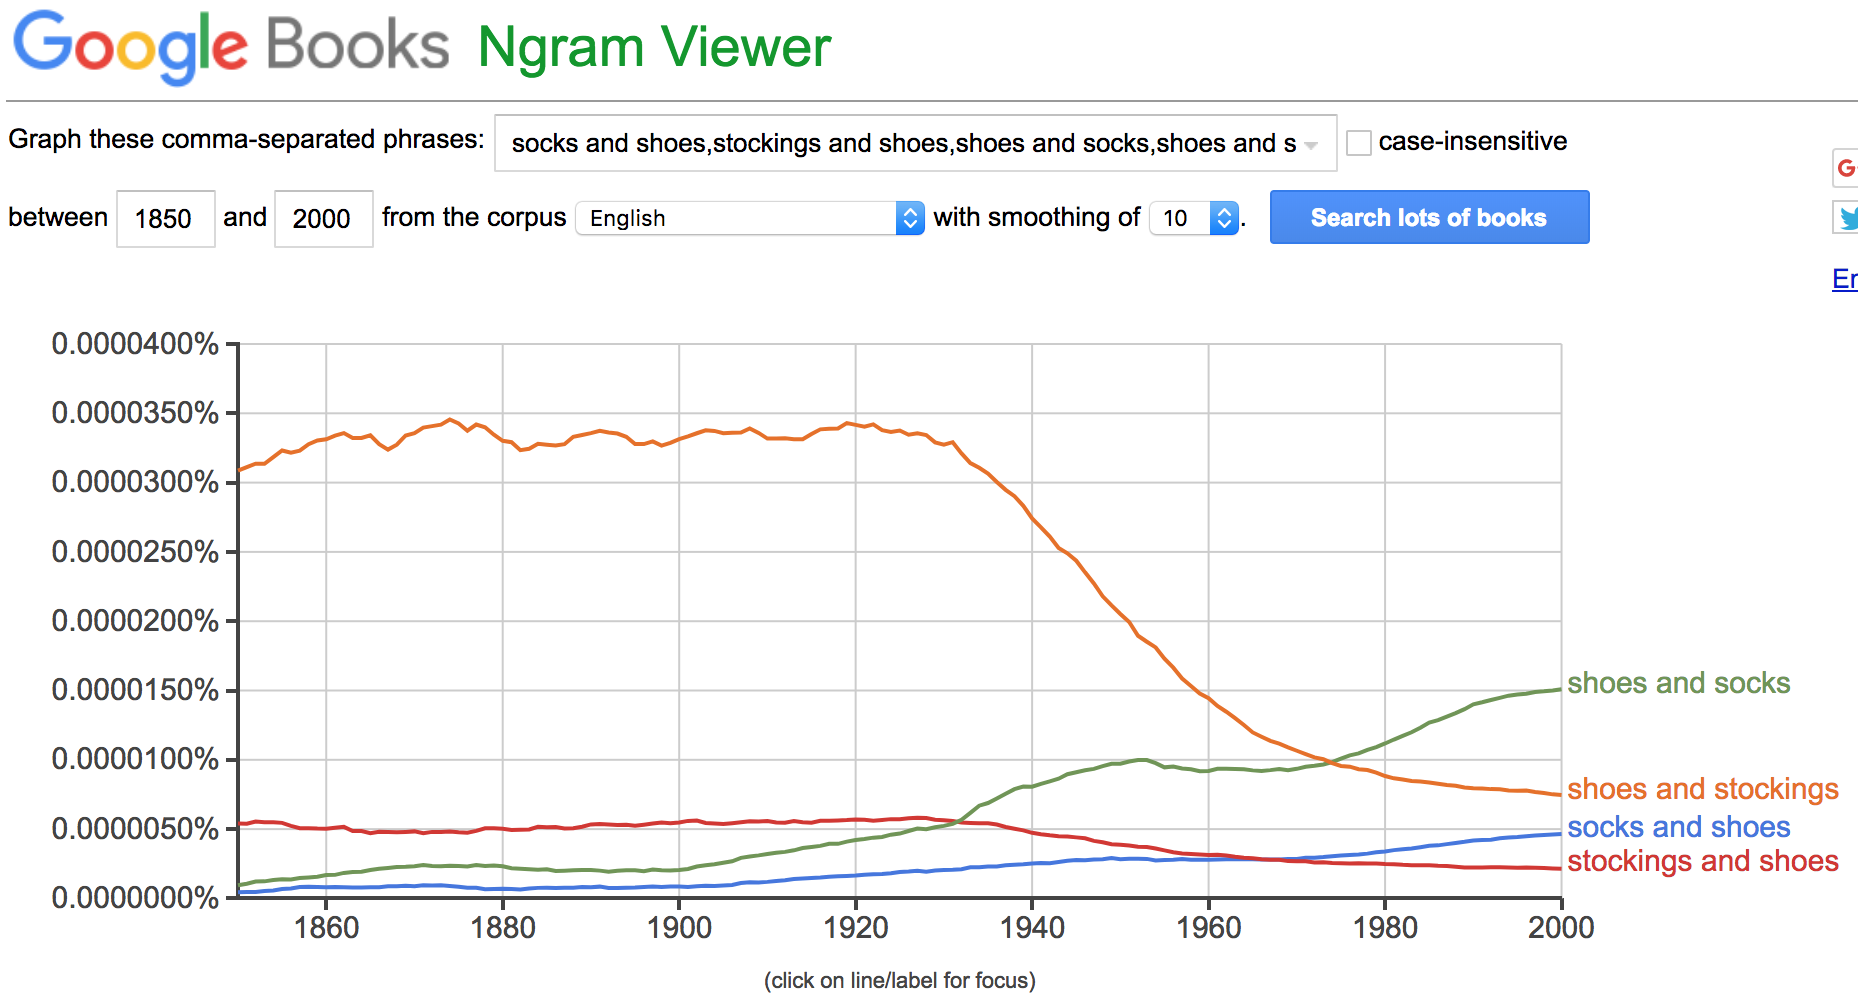
\includegraphics[width=\textwidth]{fig/google-books-stockings}}
\end{centre}

\begin{points}{Manual annotation, e.g.\ for text categorisation}
	\p Sometimes you want to split your data according to some metadata
	\begin{itemize}
			\p Can you classify literature into the year it was published?
			\p Can you classify tweets into the stated gender of the tweeter?
			\p Can you classify tweets into the stated location of the tweeter?
	\end{itemize}
	\p Sometimes you need to label a sample of documents with categories
	\begin{itemize}
			\p[\ldots] and use these categories to split a corpus and compare
			\p[\ldots] and use these categories to evaluate a classification rule
			\p[\ldots] and use these categories to train logistic regression
	\end{itemize}
	\p A \glow{gold standard} is developed by manually labelling a sample of texts
	\begin{itemize}
			\p Annotate each text multiple times, then measure \glow{inter-coder agreement}
			\p Pre-set a goal, and improve the category definitions if unmet
	\end{itemize}
\end{points}

\begin{points}{Reusing existing tools}
\p NLP focuses on accurately identifying and decoding aspects of language structure

\p Fairly mature technologies (at least in English):
\begin{itemize}
	\item identify broad categories of \glow{sentiment} expressed in a document
	\item identify \glow{topics} (words that tend to appear together) in a corpus
	\item strip inflectional \glow{morphology} from an word
	\item label each word with its \glow{part of speech}
	\item identify \glow{syntactic dependencies} between each word in a sentence
	\item identify \glow{names} of people, organisations, locations
	\item disambiguate \glow{which famous entity} is being referred to
	\item transcribe \glow{speech} to text
\end{itemize}

\item but:
\begin{itemize}
\item all these tools will make errors; use judiciously
\item may not work well on your language/medium/genre/dialect
	\end{itemize}
\end{points}


\section{Assistance}

\begin{points}{The Sydney Informatics Hub}
	\p Training and assistance in computational techniques for research
	\p \url{informatics.sydney.edu.au}
	\p a \href{https://sydney.edu.au/research/facilities.html}{Core Research Facility}

	\vfill
	\p \href{https://informatics.sydney.edu.au/services/training/}{Learn to code} for research
	\p Attend a \href{https://informatics.sydney.edu.au/hackyhour/}{Hacky Hour} for help with your research code
	\p \href{https://goo.gl/9VkMXN}{Request assistance} in collecting, analysing or modelling data
	\begin{itemize}
	\p Or: contact Chao Sun, the FASS Data Scientist
	\end{itemize}
	\vfill
	\p Are there specific techniques we should provide training in?
\end{points}

\end{document}
